\chapter[Probability and distributions]{Probability, conditional probability, diagnostic tests, discrete and normal distributions}
%VALÓSZÍNŰSÉG, FELTÉTELES VALÓSZÍNŰSÉG, DIAGNOSZTIKUS TESZTEK, DISZKRÉT ELOSZLÁSOK, NORMÁLIS ELOSZLÁS
\renewcommand{\P}{\mathrm{P}}
\section{Probability calculus}

\subsection{If we roll a dice, there are 6 possible outcomes.}
If $X$ represents the value of the outcome, find the following probabilities: 
\begin{enumerate}[a)] 
\item $\P(X = 1)=$ \hrulefill
\item $\P(X > 1)=$ \hrulefill
\item $\P(1 < X < 4)=$ \hrulefill
\end{enumerate}


\subsection{If we roll two dices, there are 36 possible outcomes.}
	\textbf{If $X$ represents the sum, $Y$ the product of the rolled numbers, find the following probabilities:}
	
	\begin{multicols}{2}	
		\begin{enumerate}[a)] 
		\item $\P(X = 2)=$ \hrulefill
		\item $\P(X > 2)=$ \hrulefill
		\item $\P(X = 10)=$ \hrulefill
		\item $\P(Y = 2)=$ \hrulefill
		\item $\P(Y = 12)=$ \hrulefill
		\end{enumerate}
		
	\columnbreak
		
	\begin{flushright}
		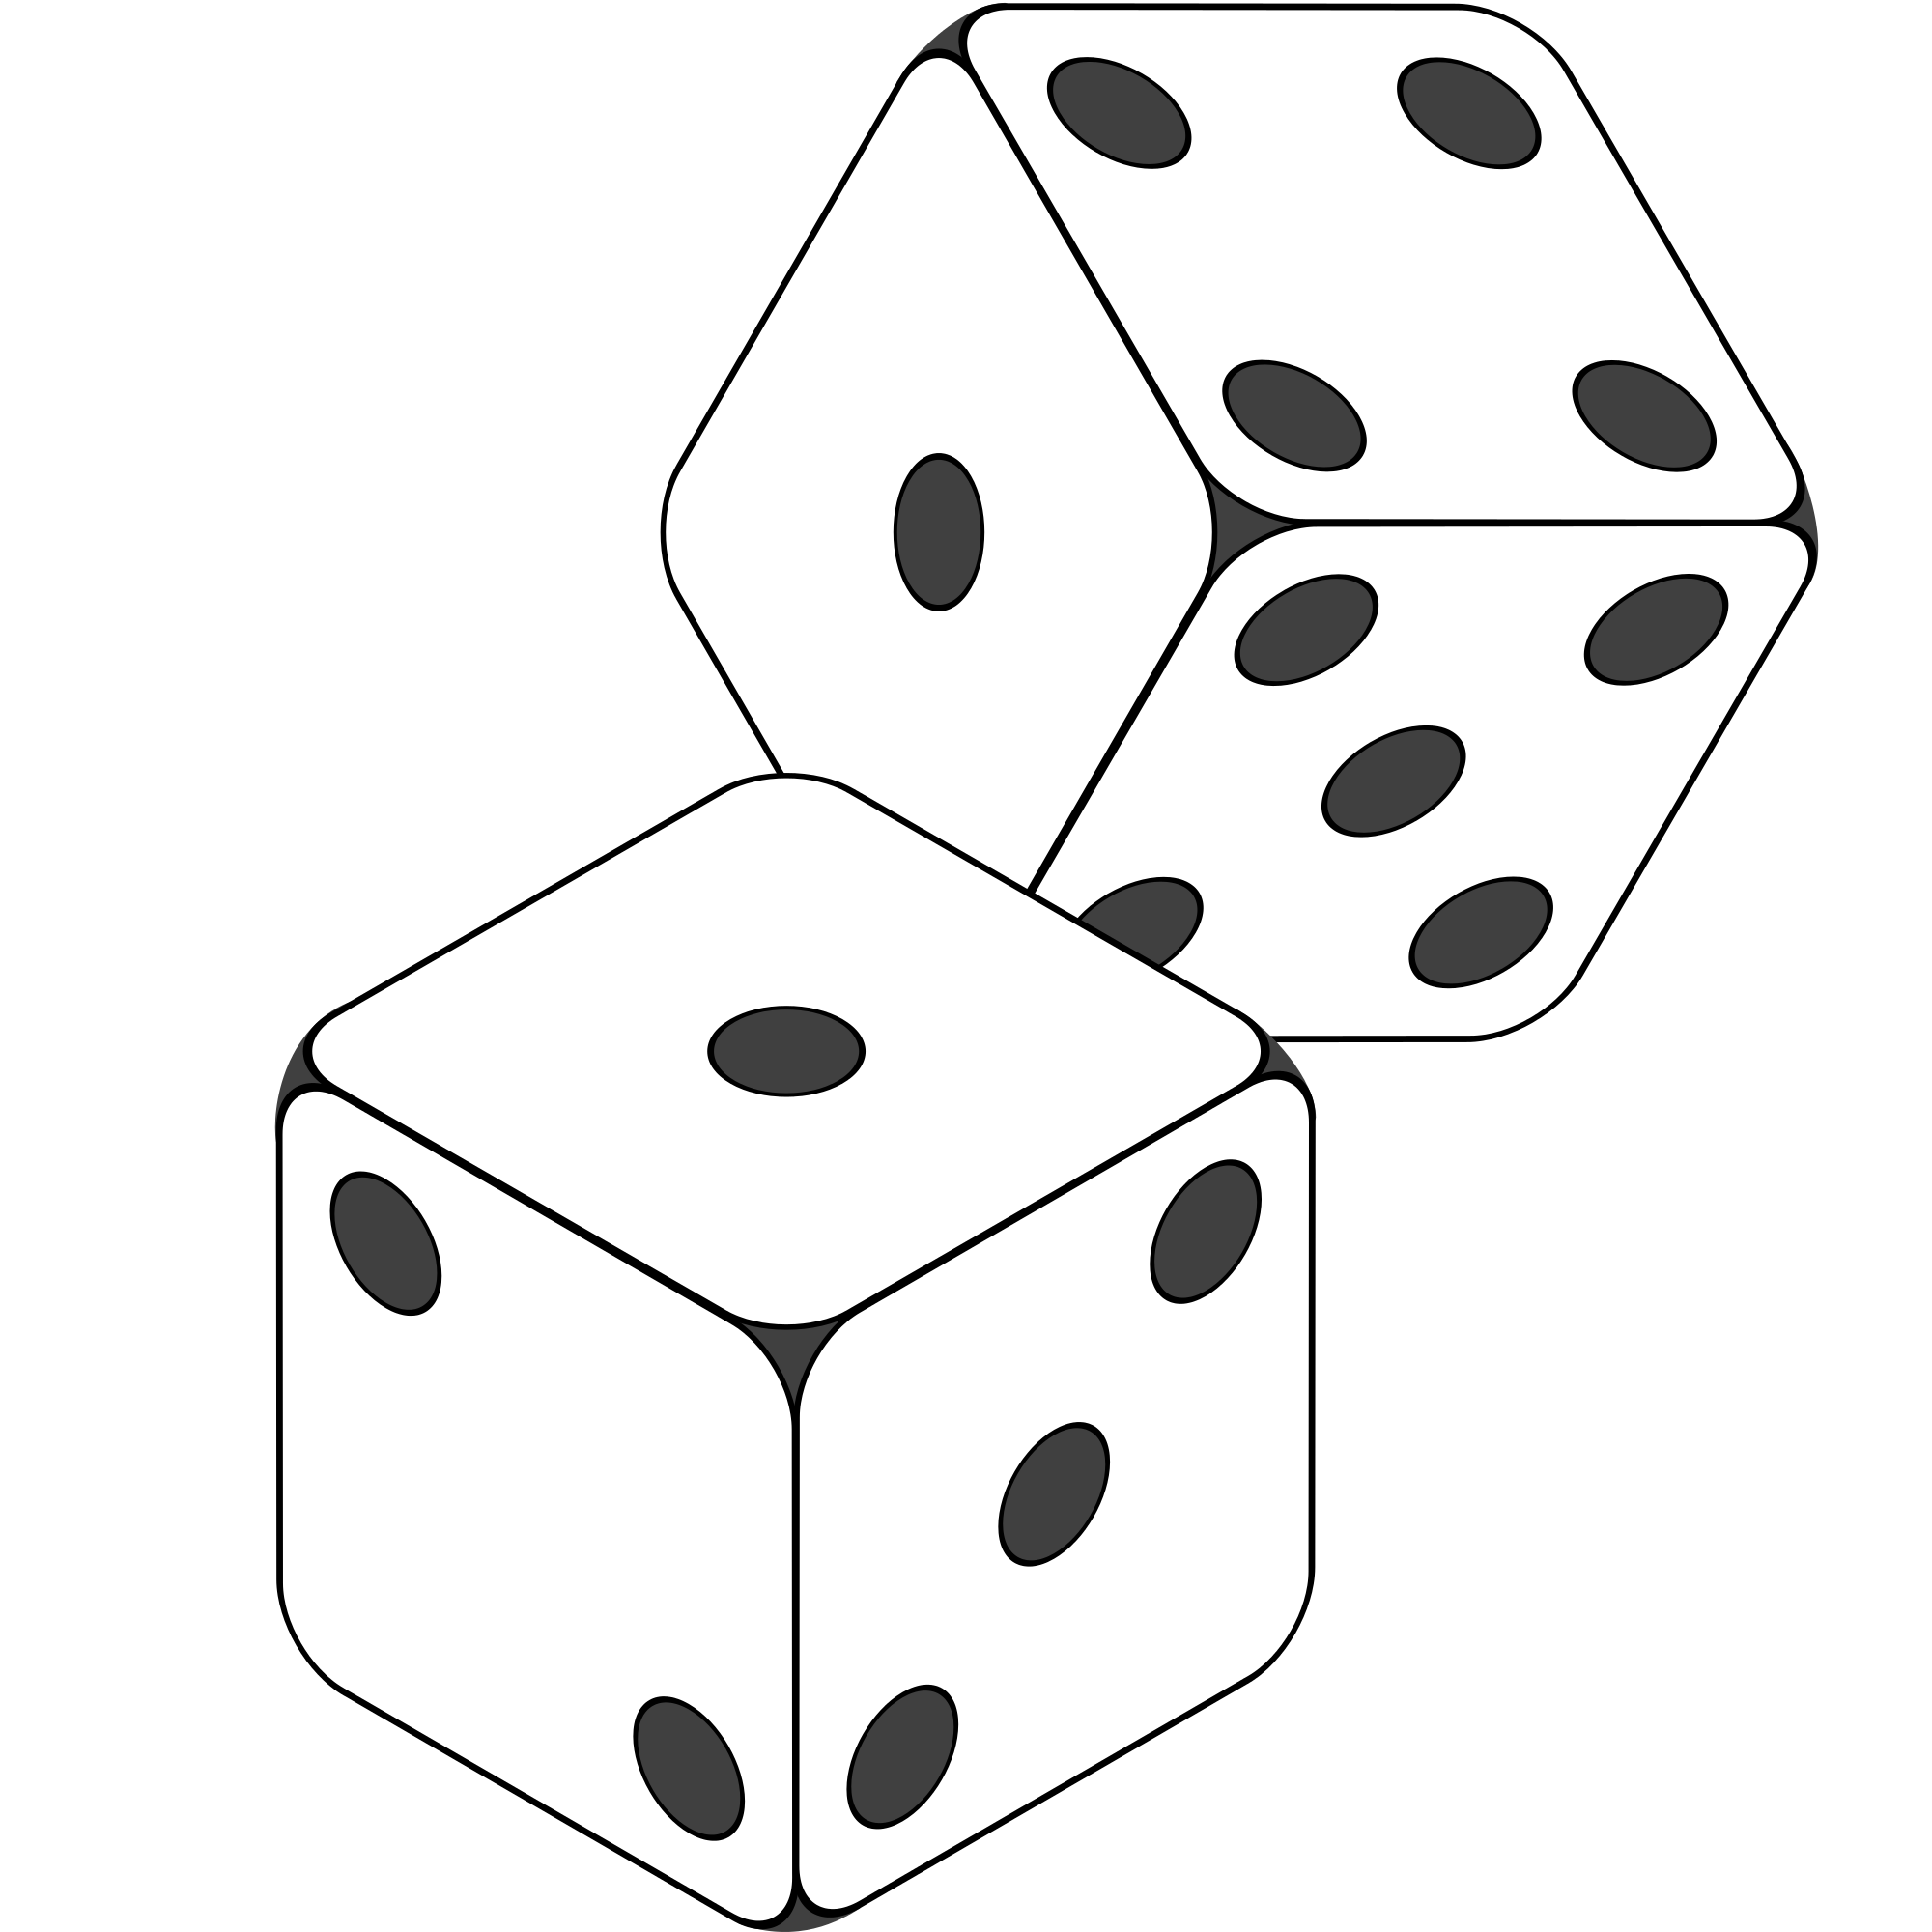
\includegraphics[width=10em]{Dice}
	\end{flushright}
	\end{multicols}	

\subsection{A fair coin is tossed twice.}


\begin{enumerate}[a)] 
\item List the possible outcomes: \hrulefill
\item Find the probability of getting two heads: \hrulefill
\end{enumerate}

\vspace{-8em}
\begin{flushright}
	\includegraphics[width=14em]{head-tail}%English_Two_Shillings_1938.jpg}
	
	head \hspace{5em} tail\hspace*{2.5em}
\end{flushright}


\subsection{A penny is tossed once and a dice is rolled once}

\begin{enumerate}[a)] 
\item List the possible outcomes: 	 \hrulefill

\textbf{Find the probabilities of the following outcomes:}
\item tossing a head and rolling an even number: \hrulefill
\item tossing a head or rolling an even number: \hrulefill
\item tossing a head and rolling a 5: \hrulefill	
\item tossing a head or rolling a 5: \hrulefill 	
\item rolling either a 4 or a 6: \hrulefill	
\end{enumerate}


%TODO ez nincs benne a magyarban
\subsection{The blood groups of 200 people are distributed as follows}
50 have blood type A, 65 have blood type B, 70 have blood type 0 and 15 have blood type AB. If a person from this group is selected at random, what is the probability that this person has blood type 0?


\section{Discrete distributions}
\subsection{A penny is tossed 3 times}
Elementary events: \hrulefill
\\
Define the variable $X$ to be the number of heads. Prepare the distribution of the variable $X$.



\newcolumntype{L}[1]{>{\raggedright\let\newline\\\arraybackslash\hspace{0pt}}m{#1}}
\newcolumntype{C}[1]{>{\centering\let\newline\\\arraybackslash\hspace{0pt}}m{#1}}
\newcolumntype{R}[1]{>{\raggedleft\let\newline\\\arraybackslash\hspace{0pt}}m{#1}}


\begin{center} 
%{\renewcommand{\arraystretch}{1.5} %<- modify value to suit your needs
	\begin{tabular}{c|C{1cm}|C{1cm}|C{1cm}|C{1cm}}
	\toprule
	$X$		& 0 & 1 & 2 & 3\\
	\midrule
	$\P(X)$ &&&&\\
	\bottomrule
	\end{tabular}
\end{center}


\subsection{Which of the following distributions are probability distributions?}
\begin{enumerate}[a)]
\item 

	\begin{tabular}{c|C{1cm}|C{1cm}|C{1cm}|C{1cm}|C{1cm}}
	\toprule
	$X$		& 0 & 5 & 10 & 15 & 20\\
	\midrule
	$\P(X)$ &1/5 &1/5&	1/5&	1/5&	1/5\\
	\bottomrule
	\end{tabular}


\item 

	\begin{tabular}{c|C{1cm}|C{1cm}|C{1cm}|C{1cm}}
	\toprule
	$X$		&0 & 2 & 	4 &	6 	\\
	\midrule
	$\P(X)$ &1/4&	1/8&	1/16&	9/16	\\
	\bottomrule
	\end{tabular}

\item 

	\begin{tabular}{c|C{1cm}|C{1cm}|C{1cm}|C{1cm}}
	\toprule
	$X$		&0 & 2 & 	4 &	6
	\\
	\midrule
	$\P(X)$ &-1& 1.5 &	0.30 & 0.2	\\
	\bottomrule
	\end{tabular}

\item	
	\begin{tabular}{c|C{1cm}|C{1cm}|C{1cm}|C{1cm}}
	\toprule
	$X$		&0 & 2 & 	4 &	6 	\\
	\midrule
	$\P(X)$ &1/4&	1/8&	1/16&	2/16	\\
	\bottomrule
	\end{tabular}	
\end{enumerate}


\section{Conditional probability}
\subsection[Conditional probability of having girls and boys]{We have large number of families with two children.  After selecting randomly a girl from this set of families estimate the probability of the event that there is a boy also in that family.}

 	
\begin{enumerate}[a)]
\item List of the elementary events: \hrulefill
\item Event $A$: \emph{there is at least one girl in the family}\quad GB, BG, GG
	\qquad
	$\P(A) =$ 	\hrulefill
\item Event $B$: \emph{there is at least one boy in the family}\quad \hrulefill
	\qquad
	$\P(B) =$ 	\hrulefill
\item Event $A$ and $B$ ($A\cdot B$): \hrulefill
	
	Possible cases from the list of elementary events: \hrulefill	
	
	$\P(AB) =$ 	\hrulefill


\item Conditional probability is $\P(B|A)= \frac{\P(AB)}{\P(A)} =$ \hrulefill	
\end{enumerate}


\subsection[Probability of 2 being rolled if the reult is even]{Calculate the probability of a 2 being rolled by a dice if it is already known that the result is even}

\noindent\hrulefill
\subsection{A dice is rolled twice, we got different numbers.}
What is the probability that at least one of them is a 6?



\noindent\hrulefill


\section{Diagnostic tests}
\subsection{Relation between results of liver scan and correct diagnosis are summarised in the following table.}
 Calculate sensitivity, specificity, positive (PPV) and negative (NPV) predictive values.

\hfill Source: D G Altman, J M Bland BMJ 1994; 308:1552


\begin{center}
	\begin{tabular}{r|cc|l}
	\toprule
			& \multicolumn{2}{c|}{\textbf{Pathology}}\\
	\textbf{Liver scan}	& abnormal (+)	& normal (-)	&Total\\
	\midrule
	abnormal (+) &	231	&32	&263\\
	normal (-)&	27	&54	&81\\
	\midrule
	Total		&258&	86	&344\\
	\bottomrule	
	\end{tabular}
\end{center}

\begin{enumerate}[a)]
\item Sensitivity: \hrulefill
\item Specificity: \hrulefill
\item PPV:	\hrulefill
\item NPV:	\hrulefill
\item Proportion of all correct diagnosis: \hrulefill
\item What does sensitivity mean? 	\hrulefill
\item What is the probability of abnormal pathology test result given abnormal liver scan result? \hrulefill
\end{enumerate}



\subsection{In the following table, the observed frequencies of two diagnostic tests are summarised. Calculate sensitivity, specificity, positive and negative predictive values.}


\begin{center}
	\begin{tabular}{r|cc|l}
	\toprule
			& \multicolumn{2}{c|}{\textbf{standard test}}\\
	\textbf{new test	}	& +	& -	&Total\\
	\midrule
	+ & 60 & 35\\
	- &	40 & 65\\
	\midrule
	Total	&&	&\\
	\bottomrule	
	\end{tabular}
\end{center}


\begin{enumerate}[a)]
\item Sensitivity: \hrulefill
\item Specificity:	\hrulefill
\item PPV:	\hrulefill
\item NPV:	\hrulefill
\item Proportion of all correct diagnosis: \hrulefill
\item What does positive predictive value (PPV) mean? 	\hrulefill
\item What is the probability of negative new test result in case of negative standard test result? \hrulefill
\end{enumerate}



\clearpage
\section{Normal distributions}

\newcommand{\N}{\mathcal{N}}
\subsection{Draw the $\N(1, 1), \N(2, 1), \N(-1, 1)$ normal distributions, if the curve of the $\N(0, 1)$ distribution is given:}

\begin{center}
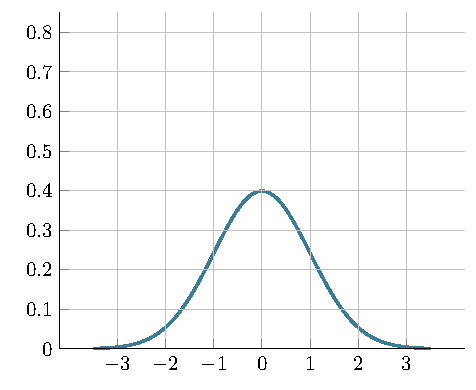
\includegraphics[height=0.37\textwidth]{03-standard-normalis}
\end{center}


\subsection{Draw the $\N(0, 2^2), \N(0, 0.5^2)$ normal distributions, if the curve of the $\N(0, 1)$ distribution is given!} 

\begin{center}
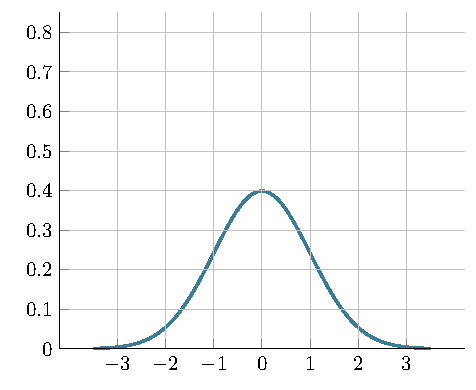
\includegraphics[height=0.37\textwidth]{03-standard-normalis}
\end{center}

\subsection{Draw the $\N(2, 2^2), \N(1, 2^2)$ normal distributions, if the curve $\N(3, 2^2)$ is given!}
\begin{center}
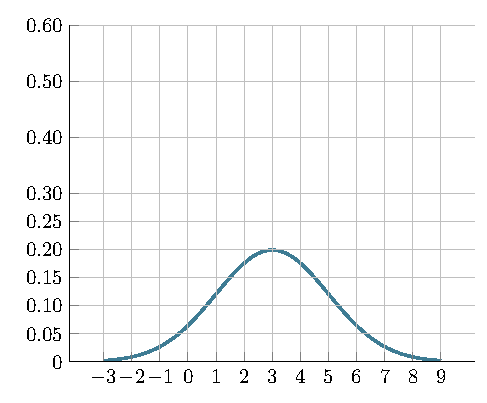
\includegraphics[height=0.37\textwidth]{03-standard-normalis2}
\end{center}



\subsection{For a standard normal distribution, find the following probabilities:}


\begin{enumerate}[a)]
\item $\P(Z < 0) =$ %Mi a valószínűsége, hogy a változó értéke 0-nál kisebb? 
	\hrulefill
\item $\P(Z > 0) =$ %Mi a valószínűsége, hogy a változó értéke 0-nál kisebb? 
	\hrulefill
\item $\P(Z < -1) =$ %Mi a valószínűsége, hogy a változó értéke -1-nél kisebb? \hrulefill	
	\hrulefill
\item $\P(Z > 1) =$ % Mi a valószínűsége, hogy a változó értéke 1-nél nagyobb?	\hrulefill
	\hrulefill
\item $\P(Z < -1,96) = 	$ \hrulefill
\item $\P(-1 < Z < 1) =$ \hrulefill
\item $\P(-1,96 < Z < 1,96) =$ \hrulefill
\item $\P(-2 < Z < 2) = $ \hrulefill
\item Find $x$ value such that the area to the left of $x$ is 0.025: \hrulefill
\item Find $x$ value such that the area to the left of $x$ is 0.5: \hrulefill
\item Which interval contains the middle 95\% of the data? \hrulefill
\item Which interval contains the middle 99\% of the data? \hrulefill
\end{enumerate}


\begin{table}[!h]\centering \small
\caption{Standard normal distribution}


 
	$\Phi(x)=\P(Z < x) =$ proportion of area to the left of $x$ (gray area)

	\begin{minipage}{0.4\textwidth}\flushright
		\begin{tabular}{ll}
		\toprule
		$x$		& $\Phi(x)$ \\
		\midrule
		$-\infty$	& $0$\footnote{limit}\\
		-4.5		& 0.00001\\
		-4		& 0.00003\\
		-3.5		& 0.00023\\
		-3		& 0.00135\\
		\midrule
		-2.576		& 0.005\\
		-2.5		& 0.00621\\
		-2.326		& 0.01\\
		-2		& 0.02275\\
		\midrule
		-1.96		& 0.025\\
		-1.645		& 0.05\\
		-1.5		& 0.06681\\
		-1		& 0.15865\\
		\midrule		
		-0.5		& 0.30854\\
		0		& 0.5\\
		0.5		& 0.69146\\
		\midrule
		1		& 0.84135\\
		1.5		& 0.93319\\
		1.645		& 0.95\\
		1.96		& 0.975\\		
		\bottomrule
		\end{tabular}\hspace{2em}
	\end{minipage}
	\begin{minipage}{0.4\textwidth}
		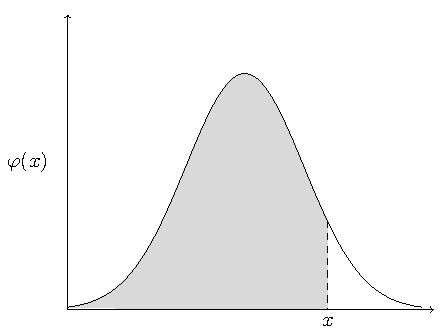
\includegraphics[width=0.95\textwidth]{03-standard-normalis-szurkitett}

		\begin{tabular}{ll}
		\toprule
		$x$		& $\Phi(x)$ \\
		\midrule
		2		& 0.97725\\
		2.326		& 0.99\\
		2.5		& 0.99379\\
		2.576		& 0.995\\
		\midrule
		3		& 0.99865\\
		3.5		& 0.99977\\
		4		& 0.99997\\
		4.5		& 0.99999\\
		$\infty$	& $1^a$\\
		\bottomrule
		\end{tabular}
		\end{minipage}		
\end{table}



\subsection{The results in a certain blood test performed in a medical laboratory are known to be normally distributed with $\N(60, 10^2)$}



\begin{enumerate}[a)]
\item What percentage of the results are below 60? 		 \hrulefill

	What percentage of the results are above 60? \hrulefill
\item What percentage of the results are between 40 and 80? 	 	 \hrulefill

What percentage of the results are below 40? 	 \hrulefill

What percentage of the results are above 80? 	 \hrulefill

\item The ''healthy range'' falls between 30 and 90. 

	What percentage of the results are between 30 and 90? \hrulefill

	What percentage of the results are outside the healthy range of 30 to 90? 	 \hrulefill
\end{enumerate}

\subsection {At an urban hospital the weights of new-born infants are normally distributed with $\N(3500, 400^2)$. Let X be the weight of a new-born picked at random. Find the following probabilities:}



\begin{enumerate}[a)]
\item $\P(X < 3500):$ \hrulefill 	
\item $\P(3100 < X < 3900):$ \hrulefill	
\item Determine the middle interval where 95\% of the weights will fall.

	 \hrulefill
\end{enumerate}


\section{Homework}

\subsection{After performing a diagnostic test we have the following frequencies:}

\begin{center}\small
	\begin{tabular}{r|cc|l}
	\toprule
			& \multicolumn{2}{c|}{\textbf{standard test}}\\
	\textbf{new test}	& +	& -	&Total\\
	\midrule
	+ & 60 & 20 & 80\\
	- &	40 & 80 & 120\\
	\midrule
	Total	&100&100	&200\\
	\bottomrule	
	\end{tabular}
\end{center}

Determine the asked proportions and give the name of the measure!
\begin{enumerate}[a)]
\item What is the proportion of people who test positive (new test +) for the disease among those who have the disease (standard test +)?\hrulefill%sensitivity


\item What is the proportion of people who test negative (new test -) for the disease among those who don't have the disease (standard test -)?
 \hrulefill% specificity


\item The proportion of the true positives among those who had positive results based on the new test?
%Az összes, az új teszt által betegnek (pozitívnak) minősített esetből mennyi a valóban betegek (valódi pozitívok) aránya?

 \hrulefill


\item The proportion of the true negatives among those who had negative results based on the new test?

\hrulefill
%Az összes, az új teszt által egészségesnek (negatívnak) minősített esetből mennyi a valóban egészséges (valódi negatívok) aránya?


\end{enumerate}

\subsection{A normal distribution has a mean of 30 and a standard deviation of 10. 
What proportion of the distribution is above 50?}
\vspace{5em}

\subsection{A ball is drawn from a box containing 10 blue balls, 10 black and 5 green. What is the probability that the ball will be green given that it is not black?}
\vfill
